\documentclass[11pt]{article}
\usepackage{amsmath}
\usepackage{amssymb}
\usepackage{graphicx}
\usepackage{fancyhdr}
\usepackage{enumerate}
\usepackage{titlesec}
\usepackage[colorlinks=true,urlcolor=blue]{hyperref}

\titlespacing{\subsubsection}{0pt}{0pt}{0pt}

% No page numbers
%\pagenumbering{gobble}

% INFORMATION SHEET (DO NOT EDIT THIS PART) ---------------------------------------------
\newcommand{\addinformationsheet}{
\clearpage
\thispagestyle{empty}
\begin{center}
\LARGE{\bf \textsf{Information sheet\\CS224W: Social and Information Network Analysis}} \\*[4ex]
\end{center}
\vfill
\textbf{Assignment Submission } Fill in and include this information sheet with each of your assignments.  This page should be the last page of your submission.  Assignments are due at 11:59pm and are always due on a Thursday.  All students (SCPD and non-SCPD) must submit their homeworks via GradeScope (\url{http://www.gradescope.com}). Students can typeset or scan their homeworks. Make sure that you answer each (sub-)question on a separate page. That is, one answer per page regardless of the answer length. Students also need to upload their code at \url{http://snap.stanford.edu/submit}. Put all the code for a single question into a single file and upload it. Please do not put any code in your GradeScope submissions. 
\\
\\
\textbf{Late Homework Policy } Each student will have a total of {\em two} free late periods. {\em Homeworks are due on Thursdays at 11:59pm PDT and one late period expires on the following Monday at 11:59pm PDT}.  Only one late period may be used for an assignment.  Any homework received after 11:59pm PDT on the Monday following the homework due date will receive no credit.  Once these late periods are exhausted, any assignments turned in late will receive no credit.
\\
\\
\textbf{Honor Code } We strongly encourage students to form study groups. Students may discuss and work on homework problems in groups. However, each student must write down their solutions independently i.e., each student must understand the solution well enough in order to reconstruct it by him/herself.  Students should clearly mention the names of all the other students who were part of their discussion group. Using code or solutions obtained from the web (github/google/previous year solutions etc.) is considered an honor code violation. We check all the submissions for plagiarism. We take the honor code very seriously and expect students to do the same. 
\vfill
\vfill
}
% ------------------------------------------------------------------------------

% MARGINS (DO NOT EDIT) ---------------------------------------------
\oddsidemargin  0.25in \evensidemargin 0.25in \topmargin -0.5in
\headheight 0in \headsep 0.1in
\textwidth  6.5in \textheight 9in
\parskip 1.25ex  \parindent 0ex \footskip 20pt
% ---------------------------------------------------------------------------------

% HEADER (DO NOT EDIT) -----------------------------------------------
\newcommand{\problemnumber}{0}
\newcommand{\myname}{name}
\newfont{\myfont}{cmssbx10 scaled 1000}
\pagestyle{fancy}
\fancyhead{}
\fancyhead[L]{\myfont Question \problemnumber, Problem Set 2, CS224W}
%\fancyhead[R]{\bssnine \myname}
\newcommand{\newquestion}[1]{
\clearpage % page break and flush floats
\renewcommand{\problemnumber}{#1} % set problem number for header
\phantom{}  % Put something on the page so it shows
}
% ---------------------------------------------------------------------------------


% BEGIN HOMEWORK HERE
\begin{document}

% Question 1.1
\newquestion{1.1}
The mean average clustering coefficient for the 100 sampled graph is $4.518\times10^{-5}$
% Question 1.2
\newquestion{1.2}
The average clustering coefficient decreases as number of iterations increases. This is reasonable because when we randomly rewrite the edges of the original graph, our graph tends more and more towards a completely random graph, which generally have much less clustering coefficient compared to a small-world graph.

\begin{figure}
\centering
  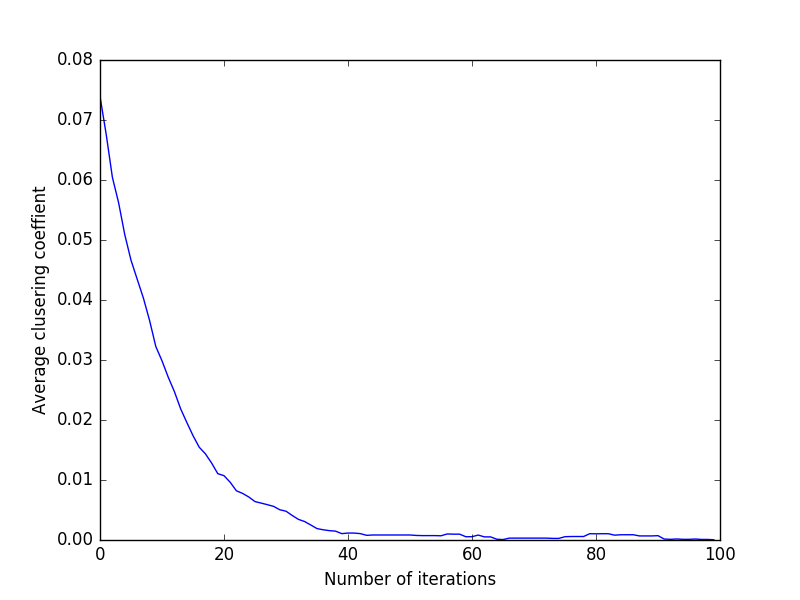
\includegraphics[width=\textwidth]{AvgClC.png}
  \caption{Average clustering coefficient V.S. Number of iterations}
  \label{Average clustering coefficient V.S. Number of iterations}
\end{figure}

% Question 2.1
\newquestion{2.1}

\subsubsection*{(a)}
The count of each type is as follows:\\
type t0: 58732\\
type t1: 396548\\
type t2: 451711\\
type t3: 4003085\\
The fraction of each type is as follows:\\
type t0: 0.01196153\\
type t1: 0.08076209\\
type t2: 0.09199674\\
type t3: 0.81527964\\

\subsubsection*{(b)}
The fraction of positive edge is :  0.8324025\\
The fraction of negative edge is:  0.1675975\\
The probability of each type:\\
type t0: $(1-p)^3=0.004707633$\\
type t1: $3p(1-p)^2=0.07014387$\\
type t2: $3p^2(1-p)=0.3483819$\\
type t3: $p^3=0.5767666$

\subsubsection*{(c)}
Type t0, t1, t3 seem to be more in the real network as calculated in (a) than in (b). \\
For t1 and t3, it's because that they are consistent with the balance theory. For t0, it's probably because there are two few of them in both (a) and (b), and the result may be subject to some variance, or the network that we are using in (a) is still under evolution, maybe eventually its t0 fraction will drop below that of (b).   

% Question 2.2
\newquestion{2.2}

\subsubsection*{(a)}
A simple lower bound for $|T|$ is $\lfloor \frac{n}{3}\rfloor$

\subsubsection*{(b)}
0.5
\subsubsection*{(c)}
The upper bound is $0.5^{\lfloor \frac{n}{3}\rfloor}$. Note that $0.5<1$ and $\lfloor \frac{n}{3}\rfloor>\frac{n}{4}$ for big $n$, let P denote the probability, we have 
\begin{align}
0&\leq \lim_{n\to\infty} P\\ 
   &\leq \lim_{n\to\infty} 0.5^{\lfloor \frac{n}{3}\rfloor}\\
   &\leq \lim_{n\to\infty} 0.5^{\frac{n}{4}}\\
   &=0
\end{align}
Therefore, we have $\lim_{n\to\infty} P=0$.

\subsubsection*{(d)}
Because in order for $G_B$ to happen, the even "all of the triangles in T are balanced" must happen, therefore $P(G_B) \leq P$, therefore $0\leq \lim_{n\to\infty} P(G_B) \leq \lim_{n\to\infty} P=0$, hence  $\lim_{n\to\infty} P(G_B)=0$
% Question 2.3
\newquestion{2.3}
No, this is not true. We can construct a counterexample as follows:

Suppose we have A, an unbalanced triad, which has 2 positive edges and 1 negative edges. And e, a positive edge of A, forms and only forms 2 extra triads with other 4 positive edges. Let B and C denote these 2 triads(Then B and C are both balanced). Then during the dynamic process, if we happen to choose A and choose e to flip, A will become balanced but B and C will become unbalanced. So the total number of balanced triads decreases by 1.

% Question 2.4
\newquestion{2.4}
$100\%$

% Question 2.5
\newquestion{2.5}
No, it's impossible. \\
Let discuss the two signs that the edge AD can take:\\
If AD is +, then in order for triad ABD and ACD to be balanced, BD and CD both must be +, but this will make triad BCD have two +(BD and CD) and one -(BC), so it's unbalanced. So AD is + is not feasible.\\
If AD is -, then in order for triad ABD and ACD to be balanced, BD and CD both must be -, but this makes triad BCD have three -, so it's unbalanced. So AD is - is not feasible, either.\\
Therefore it's impossible to add a node D such that it forms signed edges with all existing nodes (A, B, and C), but isn?t itself part of any unbalanced triangles.
% Question 2.6
\newquestion{2.6}
No, it's impossible.\\
We have proved in 2.5 that it's impossible to add a node D such that it forms signed edges with all existing nodes in a type t2 triad, but isn?t itself part of any unbalanced triangles. We now prove the same thing for type t0 triad:\\
Similar to 2.5, we denote the 3 nodes of a type t0 triad by A, B and C, respectively. Now A, B and C will all have - edges among them. Let discuss the two signs that the edge AD can take:\\
If AD is +, then in order for triad ABD and ACD to be balanced, BD and CD both must be -, but this will make triad BCD have three -, so it's unbalanced. So AD is + is not feasible.\\
If AD is -, then in order for triad ABD and ACD to be balanced, BD and CD both must be +, but this makes triad BCD have two +(BD and CD) and one -(BC), so it's unbalanced. So AD is - is not feasible, either.\\
Therefore it's impossible to add a node D such that it forms signed edges with all existing nodes (A, B, and C), but isn?t itself part of any unbalanced triangles.\\
Since for an unbalanced complete graph, there will always be at least one of two kinds of unbalanced triads(type t0 and type t2). So if a new node forms edges to all existing nodes in the unbalanced graph, it has to at least link to one triad that is either type t0 or type t1. But by doing so, the new node must be putting itself in at least on unbalanced triad, according to 2.5 and our previous proof.\\
Therefore, it is impossible for a new node X able to join the network and form edges to all existing nodes in such a way that it does not become involved in any unbalanced triangles.
% Question 3.1
\newquestion{3.1}
For graph1, B will win by 96 votes\\
For graph2, B will win by 256 votes
% Question 3.2
\newquestion{3.2}
Graph1: \$5000\\
Graph2: \$7000

\begin{figure}
\centering
  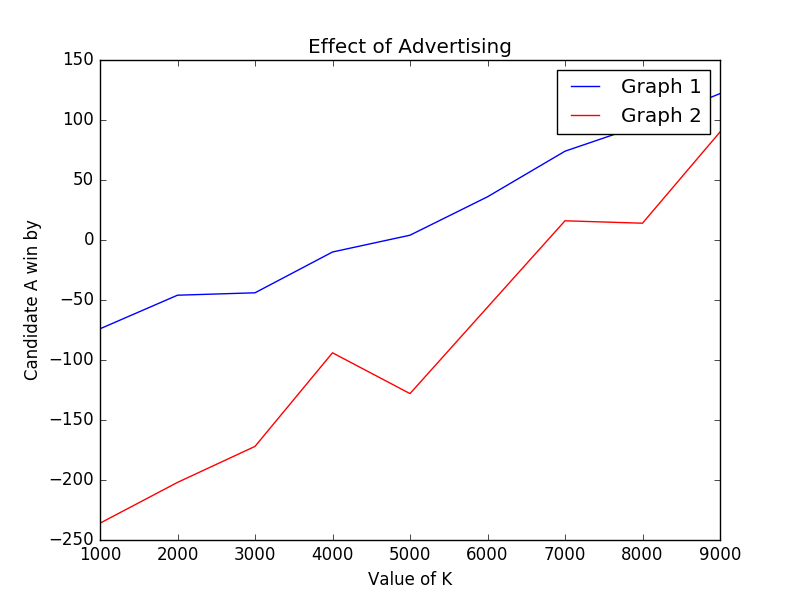
\includegraphics[width=\textwidth]{Effect_of_Advertising.png}
  \caption{Effect of Advertising}
\end{figure}


% Question 3.3
\newquestion{3.3}
Graph1 can never win. Even with \$9000, A is still down by 20 votes\\
Graph2: \$6000

\begin{figure}
\centering
  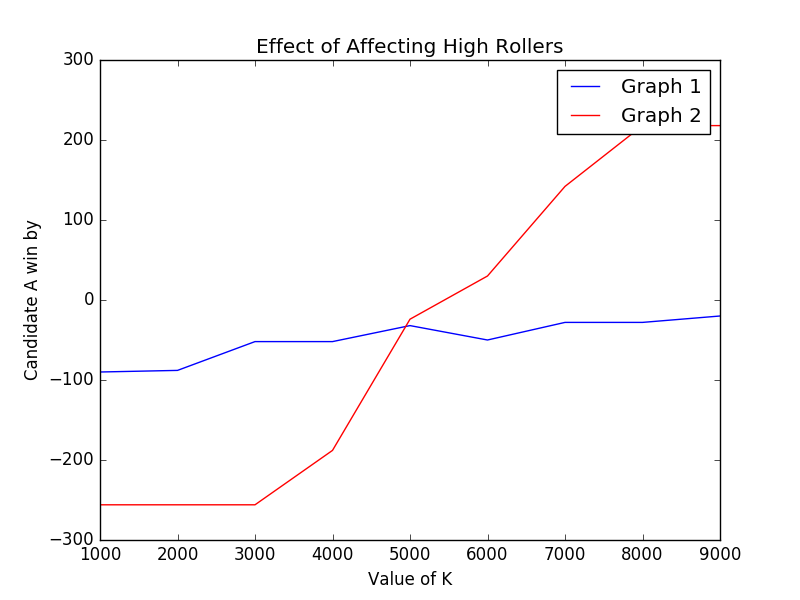
\includegraphics[width=\textwidth]{Effect_of_Affecting_High_Rollers.png}
  \caption{Effect of Affecting High Rollers}
\end{figure}
% Question 3.4
\newquestion{3.4}
\begin{figure}
\centering
  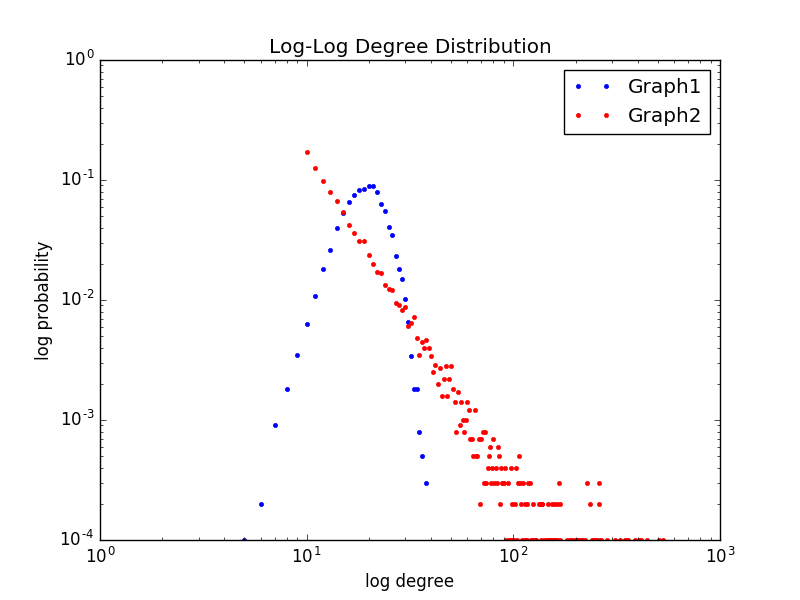
\includegraphics[width=\textwidth]{Log-Log_Degree_Distribution.png}
   \caption{Log-Log Degree Distribution}
\end{figure}

Graph 1 is Erdos-Renyi random graph and Graph2 was generated from a preferential attachment model.\\
Because in Erdos-Renyi, no nodes have very high degree, while in a preferential attachment model, some nodes tend to have very high degree. Therefore changing votes for the highest degree people will word well on a preferential attachment model and fail on Erdos-Renyi model.
% Information sheet
% Fill out the information below (this should be the last page of your assignment)
\addinformationsheet
{\Large
\textbf{Your name:}  Bowen Yao % Put your name here
\\
\textbf{Email:} boweny@stanford.edu  % Put your e-mail here
\textbf{SUID:} 06129749  % Put your student ID here
\\*[2ex] 
}
Discussion Group: None   % List your study group here
\\
\vfill\vfill
I acknowledge and accept the Honor Code.\\*[3ex]
\bigskip
\textit{BY}    % Replace this line with your initials
\vfill





\end{document}
